\documentclass{article}

\usepackage[left=1in,right=1in,top=1in,bottom=1in]{geometry}
\usepackage{epsfig}
\usepackage{amsmath}
\usepackage{subfigure}
\newcommand{\HRule}{\rule{\linewidth}{0.5mm}}
\newcommand{\Hrule}{\rule{\linewidth}{0.3mm}}

\makeatletter% since there's an at-sign (@) in the command name
\renewcommand{\@maketitle}{
  \parindent=0pt% don't indent paragraphs in the title block
  \begin{center}
    \MakeUppercase{\Large \bf \@title}
    \HRule%
  \end{center}%
  \textit{\@author \hfill \@date}
  \par
}
\makeatother% resets the meaning of the at-sign (@)

\title{System Identification for IFFL}
\author{\bf SUMIT MUKHERJEE}
\date{\bf  mukhes3@uw.edu}

\begin{document}

\maketitle% prints the title block
\vspace{5 mm}

\section{Introduction}

The aim of this work is to identify the model parameters for the different cell lines implementing the Incoherent Feed Forward Loop (IFFL). The parameters have then been used in gillespie simulations to generate stochastic trajectories.

\subsection{Identification Data Set}

Provided by Alex Rosenberg. Comprises of several cell lines :- 
\begin{itemize}
\item Open Loop 
\item Containing 4 sites complimentary to mir-124a (pv) 
\item Containing 3 sites (d3) 
\item Containing 2 sites (d23) 
\item Containing 1 site (d123) 
\end{itemize}

The data set has different time evolving values of mRNA, miRNA (both from FISH and qPCR) and protein (mCherry) levels for each of the cell lines. 

\section{Model}

Initial assumed model :- 
\begin{align*}
\frac{dm}{dt} &= \alpha_{m} - \beta_m m - \gamma_s m s \\
\frac{ds}{dt} &= \alpha_s - \beta_s s \\
\frac{dp}{dp} &= \alpha_p m - \beta_p p  
\end{align*}

Where, $m$ is the mRNA concentration, $s$ is the miR-124a concentration, $p$ is the protein concentration, $\alpha_m$ is mRNA production rate, $\alpha_s$ is the miRNA production rate, $\alpha_p$ is the protein production rate (not constitutive), $\beta_m$ is the mRNA degradation rate, $\beta_s$ is the miRNA degradation rate, $\beta_p$ is the protein degradation rate and $\gamma_s$ is the miRNA degradation rate for mRNA. 

\section{Parameter Identification}

\subsection{Cost Function}
We observe that the time evolution of the miRNA is independent of the mRNA and protein concentration, so we identify it separately and club the mRNA and protein into one identification routine.  The cost function used is :- 
\begin{align*}
J = \sum\limits_{j = 1}^{j = l}  a_j \sum\limits_{i = 1}^{i = k} \frac{{(x_{j}(i) - x_{act,j}(i))}^2}{{x_{act,j}(k)}^2} 
\end{align*}
Where, $x_j(i)$ represents the simulated concentration of $j$th specie at $i$th time point, $x_{act,j}(i)$ represents the actual concentration of $j$th specie at $i$th time point, $k$ is the number of time points, $l$ is the number of species and $a_j$ is the weight on the $j$th specie. The term in the denominator ensures that the species get normalized (as mRNA, protein and miRNA concentrations are often vastly different). The parameters being optimized here are $\alpha_m, \alpha_s, \alpha_p, \beta_m, \beta_s, \beta_p, \gamma_s$.   

\subsection{Parameter Limits}

The decay rate limits are chosen based on practical values of half lifes and are chosen to be within one order of magnitude each way. The maximal limit on the production limit is chosen to be a realistic value based on the plots. The limits used for the various parameters are given in Table~\ref{MinMaxTable} :- 

\begin{table}[h!]
\begin{center}
\begin{tabular}{|l|l|l|}
\hline
Parameter & Min & Max \\\hline
$\beta_m$ (1/h) &.01 &.5 \\\hline
$\beta_s$ (1/h) &.02 &.04 \\\hline 
$\beta_p$ (1/h) &.001 &1 \\\hline 
$\alpha_m$ (conc./h) &100 &3000 \\\hline
$\alpha_s$ (conc./h) &0 &500 \\\hline
$\alpha_p$ (1/h) &0 &5000 \\\hline
$\gamma_s$ (1/h conc.) &0 &.00001 \\\hline 
\end{tabular}
\end{center}
\caption{Minimum and Maximum values of parameters}
\label{MinMaxTable}
\end{table}

\subsection{Identified Parameters}

The identified parameters are given in Table~\ref{paramTable}.

\begin{table}[h!]
\begin{center}
\begin{tabular}{|l|l|l|l|l|l|}
\hline
Parameter & PV & d3 & d23 & d123 & in paper\\\hline
$\beta_m$ (1/h) &0.26645&0.13174&0.5&0.21695 &.1\\\hline
$\beta_s$ (1/h) &0.029091&0.028633&0.02363&0.04 & .03\\\hline
$\beta_p$ (1/h) &0.054131&0.03673&0.030614&0.018773 & .08\\\hline
$\alpha_m$ (conc./h) &524.9764&517.0953&208.5493&270.1188 &0-150\\\hline
$\alpha_s$ (conc./h) &50.0004&70.7653&22.036&49.0797 & 0-60\\\hline
$\alpha_p$ (1/h) &1.5638&1.1415&3.3885&1.6738 & 10\\\hline
$\gamma_s$ (1/h conc.) &0.001&0.00051711&0.00097197&0.00028637 & .00075\\\hline
\end{tabular}
\end{center}
\caption{Identified values for different parameters}
\label{paramTable}
\end{table}

\subsection{Plots}
The plots for each of the classes are shown below :- 
\begin{figure}[h!]
\centering
\subfigure[]{\includegraphics[scale=.1]{IFFL_Alex_pv/model4mRNAcont.jpg}}
\subfigure[]{\includegraphics[scale=.1]{IFFL_Alex_pv/model4miRNAcont.jpg}}
\subfigure[]{\includegraphics[scale=.1]{IFFL_Alex_pv/model4pcont.jpg}}
\caption{Simulation vs Real plots for PV : a) mRNA b) miRNA (mir-124a) c) protein (mCherry)}
\label{resultsPV}
\end{figure}

\begin{figure}[h!]
\centering
\subfigure[]{\includegraphics[scale=.1]{IFFL_Alex_d3/model4mRNAcont.jpg}}
\subfigure[]{\includegraphics[scale=.1]{IFFL_Alex_d3/model4miRNAcont.jpg}}
\subfigure[]{\includegraphics[scale=.1]{IFFL_Alex_d3/model4pcont.jpg}}
\caption{Simulation vs Real plots for d3 : a) mRNA b) miRNA (mir-124a) c) protein (mCherry)}
\label{resultsd3}
\end{figure}

\begin{figure}[h!]
\centering
\subfigure[]{\includegraphics[scale=.1]{IFFL_Alex_d23/model4mRNAcont.jpg}}
\subfigure[]{\includegraphics[scale=.1]{IFFL_Alex_d23/model4miRNAcont.jpg}}
\subfigure[]{\includegraphics[scale=.1]{IFFL_Alex_d23/model4pcont.jpg}}
\caption{Simulation vs Real plots for d23 : a) mRNA b) miRNA (mir-124a) c) protein (mCherry)}
\label{resultsd23}
\end{figure}

\begin{figure}[h!]
\centering
\subfigure[]{\includegraphics[scale=.1]{IFFL_Alex_d123/model4mRNAcont.jpg}}
\subfigure[]{\includegraphics[scale=.1]{IFFL_Alex_d123/model4miRNAcont.jpg}}
\subfigure[]{\includegraphics[scale=.1]{IFFL_Alex_d123/model4pcont.jpg}}
\caption{Simulation vs Real plots for d123 : a) mRNA b) miRNA (mir-124a) c) protein (mCherry)}
\label{resultsd123}
\end{figure}

\pagebreak

\subsection{Open Loop Plots and Parameters}

Table~\ref{paramTableOpenFish} shows the values of the parameters identified with the open loop data (the mRNA data is used from the FISH data for open loop). The plots of the open loop identification are shown below in Figure~\ref{resultsP}. 


\begin{table}[h!]
\begin{center}
\begin{tabular}{|l|l|}
\hline
Parameter & P \\\hline
$\beta_m$ (1/h) &0.3169\\\hline
$\beta_s$ (1/h) &0.0247\\\hline
$\beta_p$ (1/h) &0.0201\\\hline
$\alpha_m$ (conc./h) &140.7183\\\hline
$\alpha_s$ (conc./h) &51.0592\\\hline
$\alpha_p$ (1/h) &6.5936\\\hline
$\gamma_s$ (1/h conc.) &0\\\hline
\end{tabular}
\end{center}
\caption{Identified values for different parameters}
\label{paramTableOpenFish}
\end{table}

\begin{figure}[h!]
\centering
\subfigure[]{\includegraphics[scale=.1]{IFFL_Alex_p_FISH/model4mRNAcont.jpg}}
\subfigure[]{\includegraphics[scale=.1]{IFFL_Alex_p_FISH/model4miRNAcont.jpg}}
\subfigure[]{\includegraphics[scale=.1]{IFFL_Alex_p_FISH/model4pcont.jpg}}
\caption{Simulation vs Real plots for P (open loop) : a) mRNA b) miRNA (mir-124a) c) protein (mCherry)}
\label{resultsP}
\end{figure}

\subsection{Re-identification with FISH data}

We have mRNA data from FISH (Fluorescence in situ hybridization) for both P (open loop) and  PV cell lines. The re-identification of the PV cell line yields the parameter values as seen in table and the plots can be seen in figure 


\begin{table}[h!]
\begin{center}
\begin{tabular}{|l|l|}
\hline
Parameter & P \\\hline
$\beta_m$ (1/h) &0.2615\\\hline
$\beta_s$ (1/h) &0.0290\\\hline
$\beta_p$ (1/h) &0.0514\\\hline
$\alpha_m$ (conc./h) &194.9786\\\hline
$\alpha_s$ (conc./h) &49.967\\\hline
$\alpha_p$ (1/h) &3.9719\\\hline
$\gamma_s$ (1/h conc.) &0\\\hline
\end{tabular}
\end{center}
\caption{Identified values for different parameters}
\label{paramTableOpenFish}
\end{table}

\begin{figure}[h!]
\centering
\subfigure[]{\includegraphics[scale=.1]{IFFL_Alex_pv_FISH/model4mRNAcont.jpg}}
\subfigure[]{\includegraphics[scale=.1]{IFFL_Alex_pv_FISH/model4miRNAcont.jpg}}
\subfigure[]{\includegraphics[scale=.1]{IFFL_Alex_pv_FISH/model4pcont.jpg}}
\caption{Simulation vs Real plots for PV : a) mRNA b) miRNA (mir-124a) c) protein (mCherry)}
\label{resultsPV_Fish}
\end{figure}

\subsection{Open loop plots with PV-FISH parameters}

Theoretically, the open loop plot can be obtained by setting $gs = 0$ and making the initial conditions to be the same as the initial conditions for the open loop case. This yields the plots seen in Figure~\ref{resultsPV_FishOpen}.  

\begin{figure}[h!]
\centering
\subfigure[]{\includegraphics[scale=.1]{IFFL_Alex_pv_FISH/model4mRNAopencont.jpg}}
\subfigure[]{\includegraphics[scale=.1]{IFFL_Alex_pv_FISH/model4miRNAopencont.jpg}}
\subfigure[]{\includegraphics[scale=.1]{IFFL_Alex_pv_FISH/model4popencont.jpg}}
\caption{Simulation vs Real plots for PV : a) mRNA b) miRNA (mir-124a) c) protein (mCherry)}
\label{resultsPV_FishOpen}
\end{figure}
 
Clearly this does not lead to very well fitted plots. We assume that this could be a result of a translation inhibition. If only that was the case, the mRNA levels would roughly remain the same but the steady state value seems of the open loop case seems to be around half the steady state value of the PV cell line. Hence we fix all other parameters and just vary $\alpha_p$ and $\alpha_m$ to see if we can better fits. The plots obtained are shown in figure 

\begin{figure}[h!]
\centering
\subfigure[]{\includegraphics[scale=.1]{IFFL_Alex_pv_FISH/model4mRNAopencontupdated.jpg}}
\subfigure[]{\includegraphics[scale=.1]{IFFL_Alex_pv_FISH/model4miRNAopencontupdated.jpg}}
\subfigure[]{\includegraphics[scale=.1]{IFFL_Alex_pv_FISH/model4popencontupdated.jpg}}
\caption{Simulation vs Real plots for PV : a) mRNA b) miRNA (mir-124a) c) protein (mCherry)}
\label{resultsPV_FishUpdated}
\end{figure}

The identified values of parameters are shown in table 

\begin{table}[h!]
\begin{center}
\begin{tabular}{|l|l|}
\hline
Parameter & P \\\hline
$\alpha_m$ (conc./h) &104.91\\\hline
$\alpha_p$ (1/h) &11.3891\\\hline
\end{tabular}
\end{center}
\caption{Identified values for different parameters}
\label{paramTableOpenFishUpdated}
\end{table}

This yields slightly better fits. However, we are interested to see whether this is just due to cell line variability or whether translation inhibition has a role to play here. So, now we just vary the $\alpha_m$ (change it to re-identified value) and keep everything else fixed (to the first case) and observe the results in Figure  

\begin{figure}[h!]
\centering
\subfigure[]{\includegraphics[scale=.1]{IFFL_Alex_pv_FISH/model4mRNAopencontupdated2.jpg}}
\subfigure[]{\includegraphics[scale=.1]{IFFL_Alex_pv_FISH/model4miRNAopencontupdated2.jpg}}
\subfigure[]{\includegraphics[scale=.1]{IFFL_Alex_pv_FISH/model4popencontupdated2.jpg}}
\caption{Simulation vs Real plots for PV : a) mRNA b) miRNA (mir-124a) c) protein (mCherry)}
\label{resultsPV_FishUpdated}
\end{figure}

So clearly, there is translation inhibition happening which causes the $\alpha_p$ value to be higher in the re-identified case. 

%\section{Stochastic Simulations}
%
%Stochastic simulations were performed on the Control and Full Vamp3 strains using the Tau Leaping method to calculated the statistics. The obtained images are shown below :- 
%\begin{figure}[h!]
%\centering 
%\subfigure[]{\includegraphics[scale=.1]{TauL_IFFL_FISH_p/m}}
%\subfigure[]{\includegraphics[scale=.1]{TauL_IFFL_FISH_p/s}}
%\subfigure[]{\includegraphics[scale=.1]{TauL_IFFL_FISH_p/p}}
%\subfigure[]{\includegraphics[scale=.1]{TauL_IFFL_FISH_pv/m}}
%\subfigure[]{\includegraphics[scale=.1]{TauL_IFFL_FISH_pv/s}}
%\subfigure[]{\includegraphics[scale=.1]{TauL_IFFL_FISH_pv/p}}
%\caption{Tau Leaping plots for Control : a) mRNA b) miRNA (mir-124a) c) protein (mCherry), Tau Leaping plots for Full Vamp3 : a) mRNA b) miRNA (mir-124a) c) protein (mCherry)}
%\label{stochPV_FishUpdated}
%\end{figure}


\section{Identification at multiple Dox levels}

Protein 
fluorescence data from at different Dox induction levels was available for various cell lines. Unfortunately the miRNA and mRNA time course data aren't available. Thus the problem reduces to finding
the initial conditions along with the parameters. However, it is expected that the other parameters remain
the same and only the $a_m$ and $b_m$ varies. However, their ratio is assumed to be constant, so we need to only identify $a_m$ for different Dox level. So, the optimization variables are m0, s0 and $a_m$. The plots for the
protein fits is seen in Figure~\ref{MultiDoxFits} for the Full Vamp3 cell line. The predicted plot for 
fluorescence and mRNA levels at different
Dox induction levels is shown in the Figure~\ref{MultiDoxpredict}.

\begin{figure}[h!]
\centering
\subfigure[]{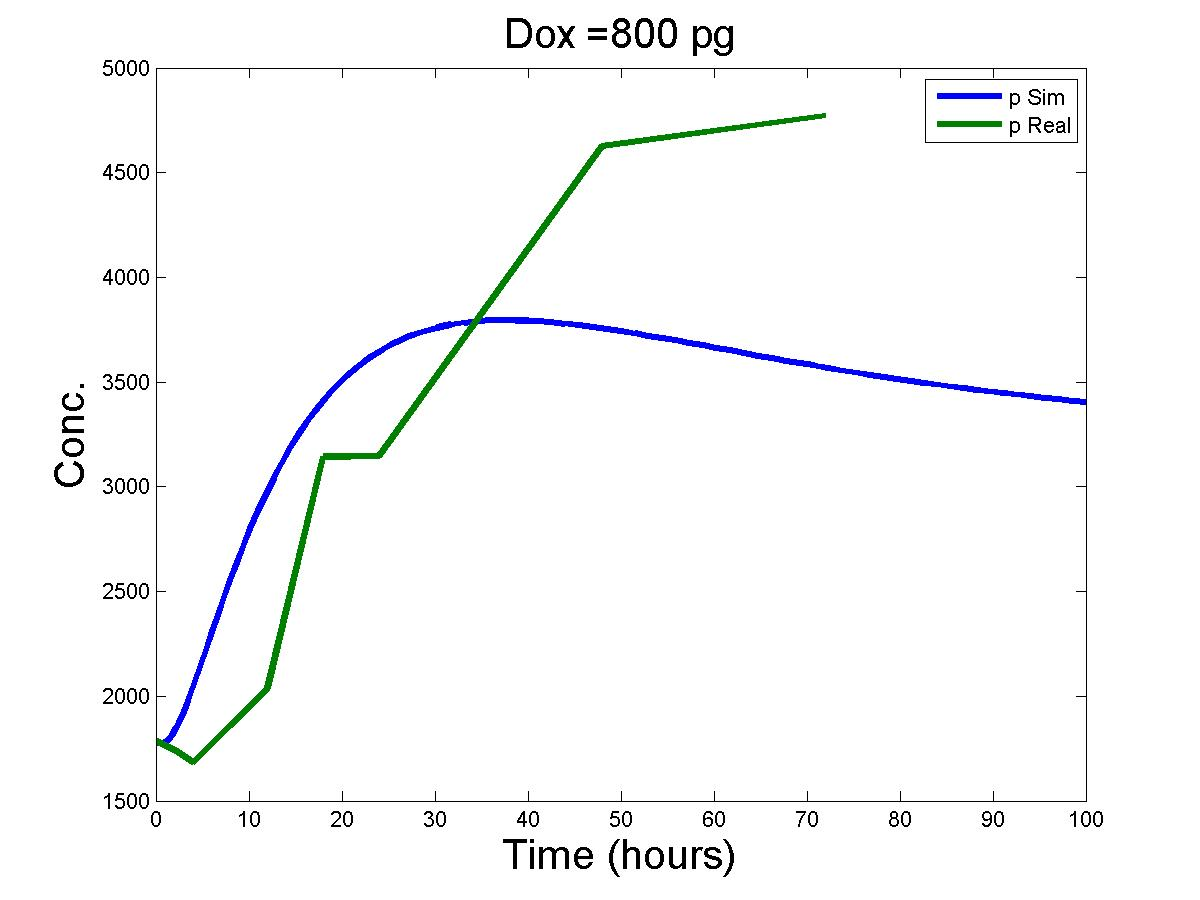
\includegraphics[scale=.1]{MultiDox_pv_mod/Dox800pCont}}
\subfigure[]{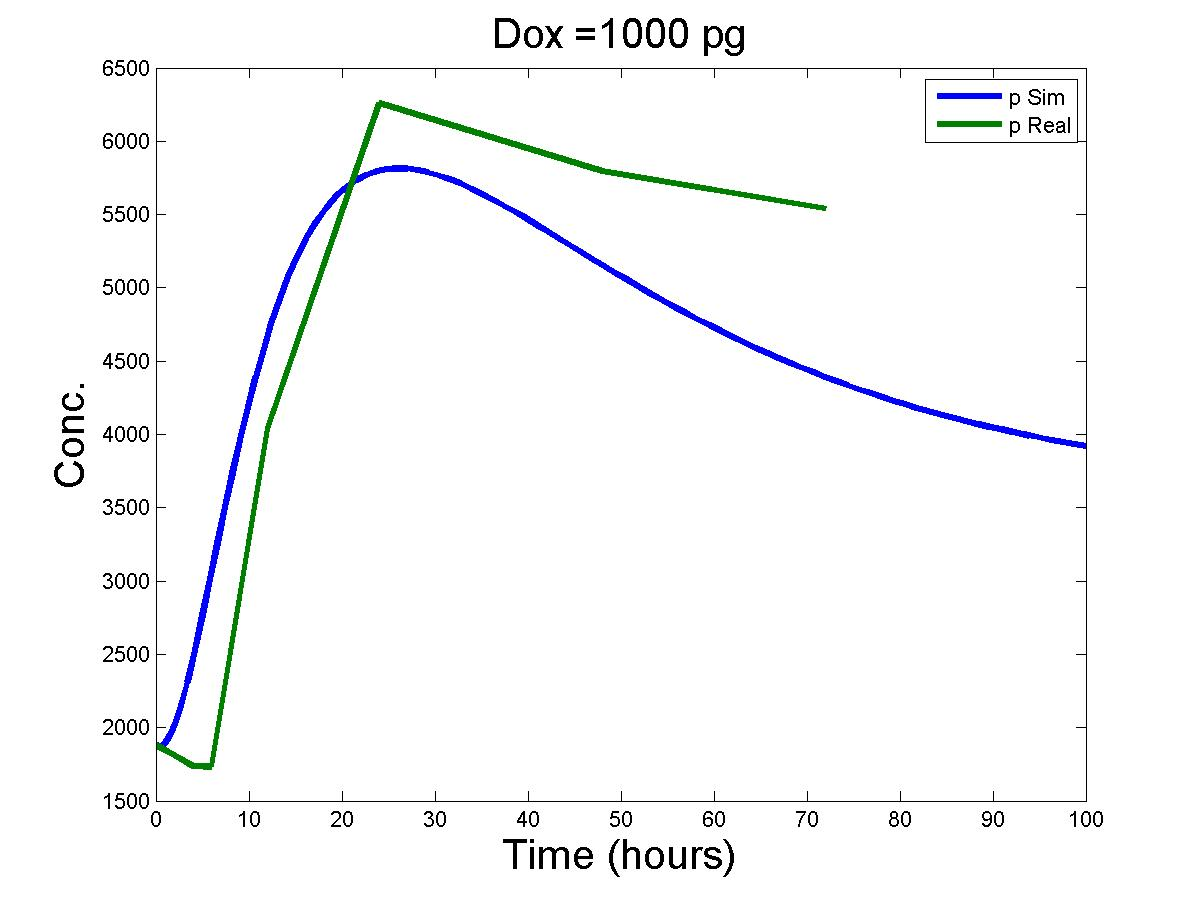
\includegraphics[scale=.1]{MultiDox_pv_mod/Dox1000pCont}}
\subfigure[]{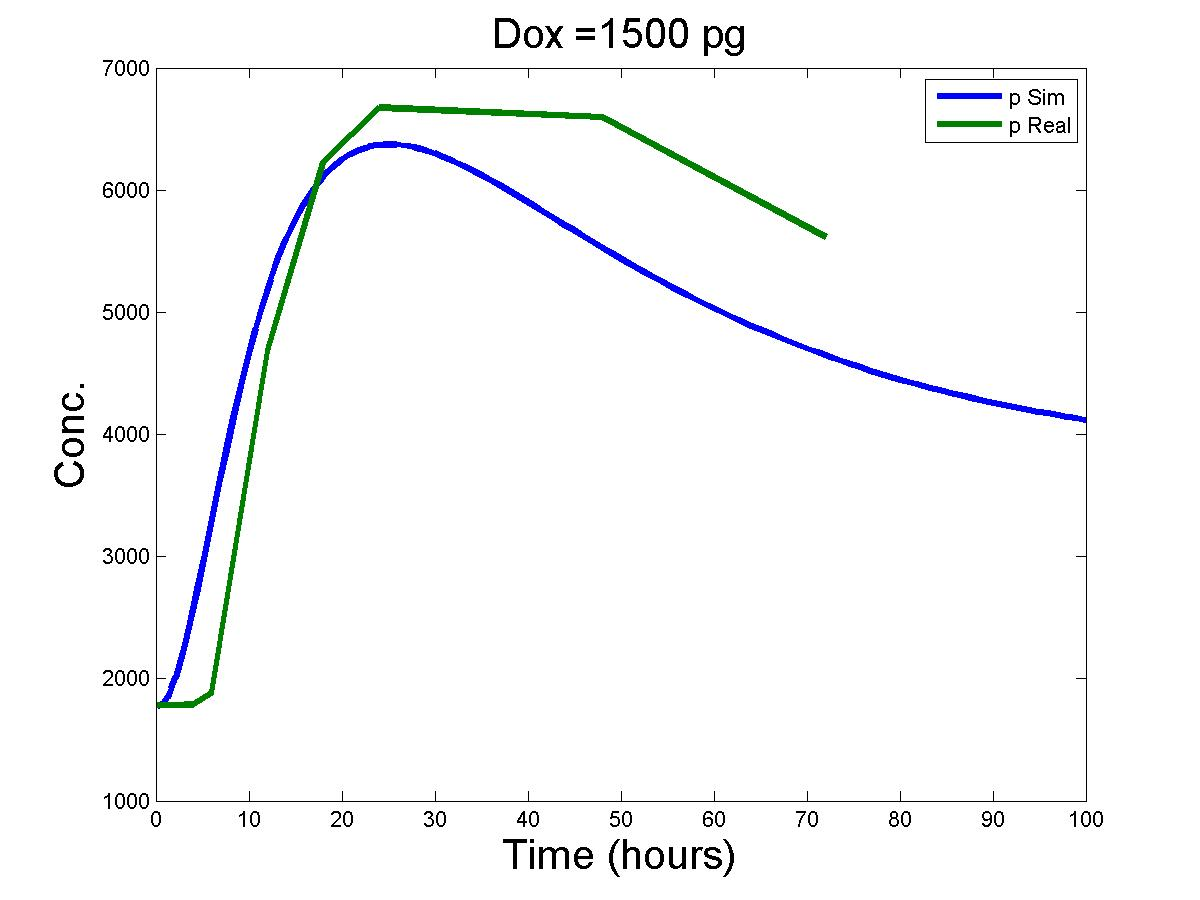
\includegraphics[scale=.1]{MultiDox_pv_mod/Dox1500pCont}}
\subfigure[]{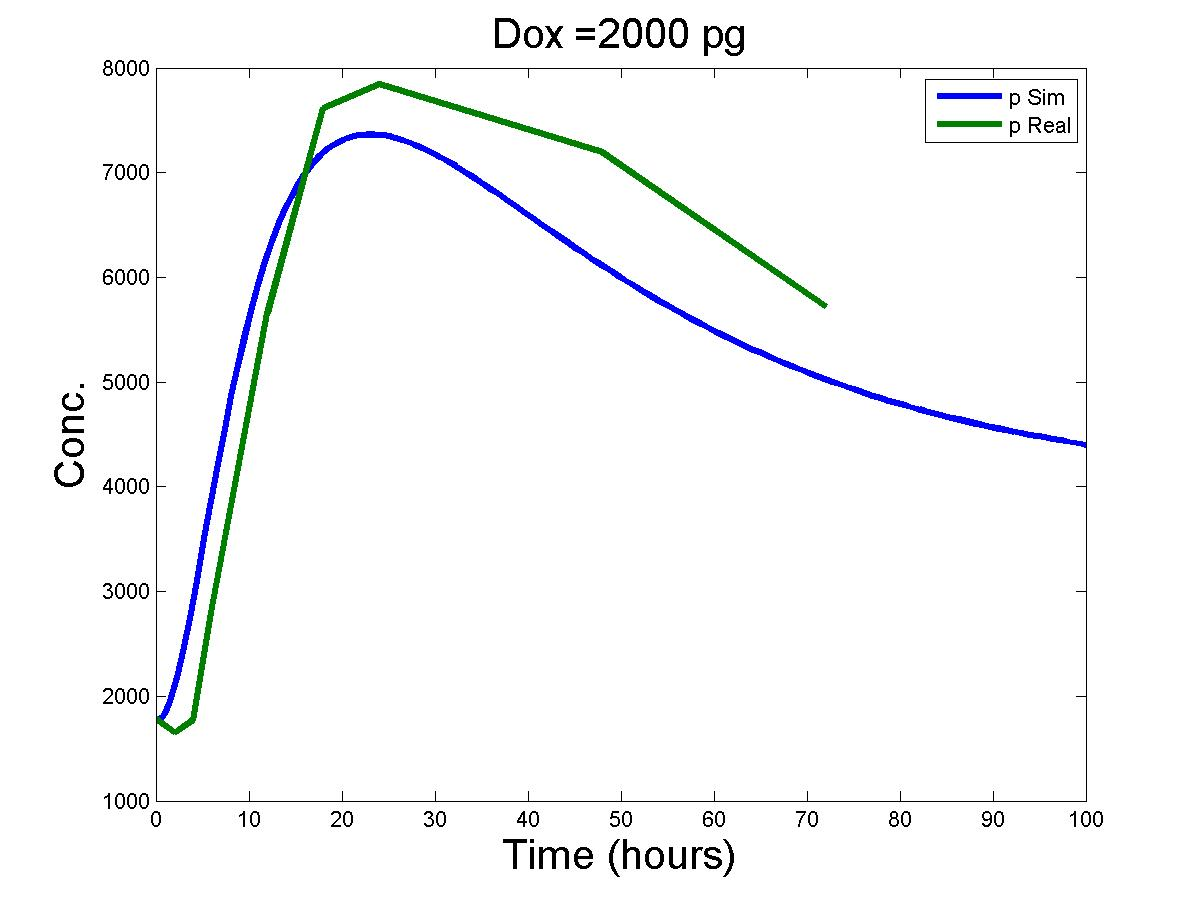
\includegraphics[scale=.1]{MultiDox_pv_mod/Dox2000pCont}}
\subfigure[]{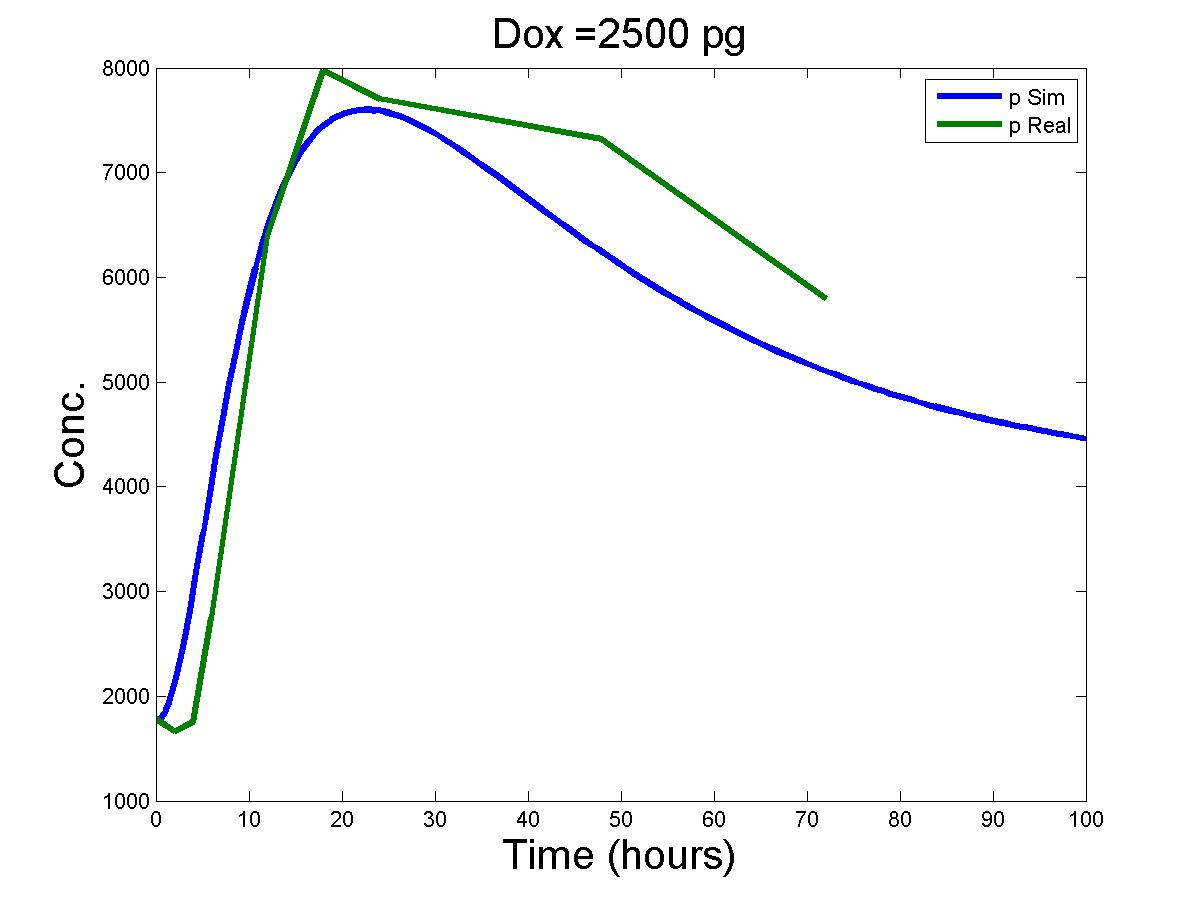
\includegraphics[scale=.1]{MultiDox_pv_mod/Dox2500pCont}}
\subfigure[]{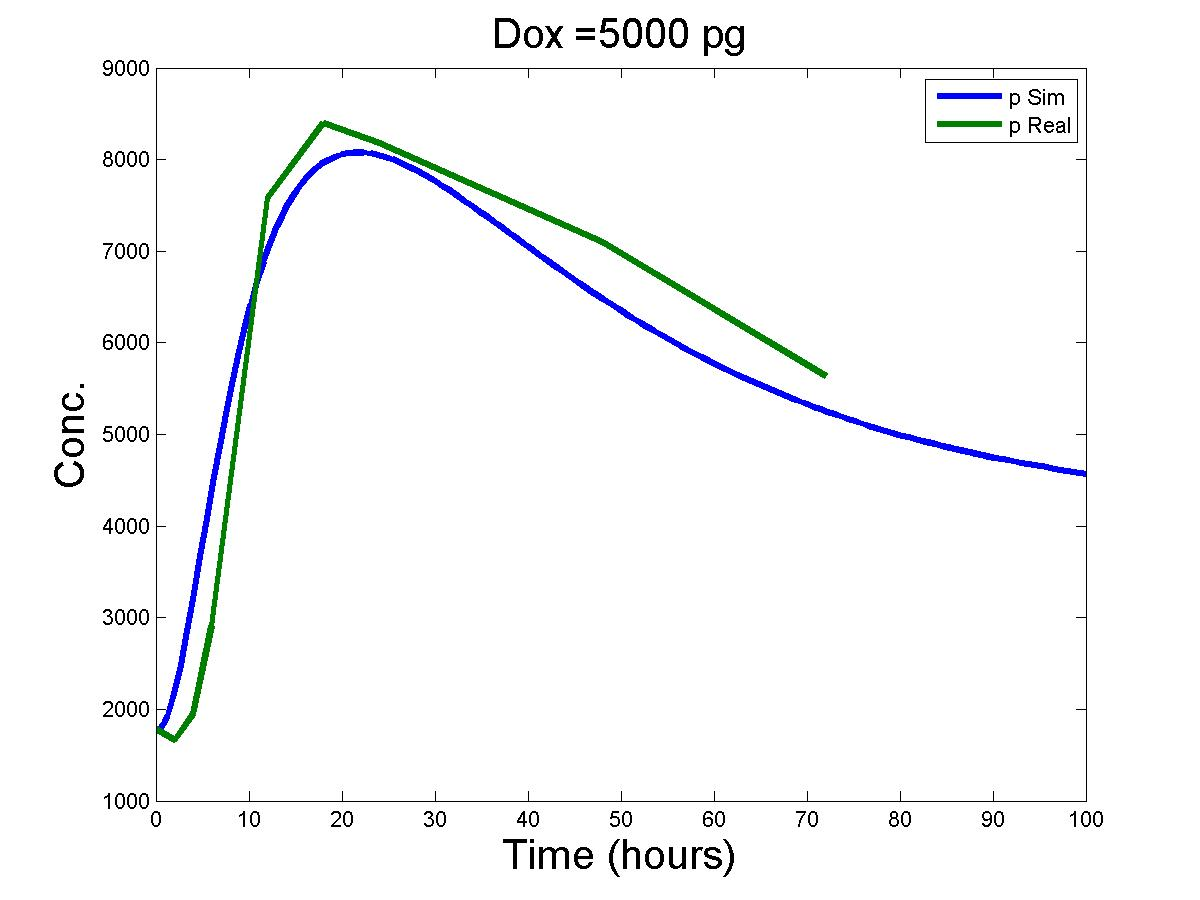
\includegraphics[scale=.1]{MultiDox_pv_mod/Dox5000pCont}}
\subfigure[]{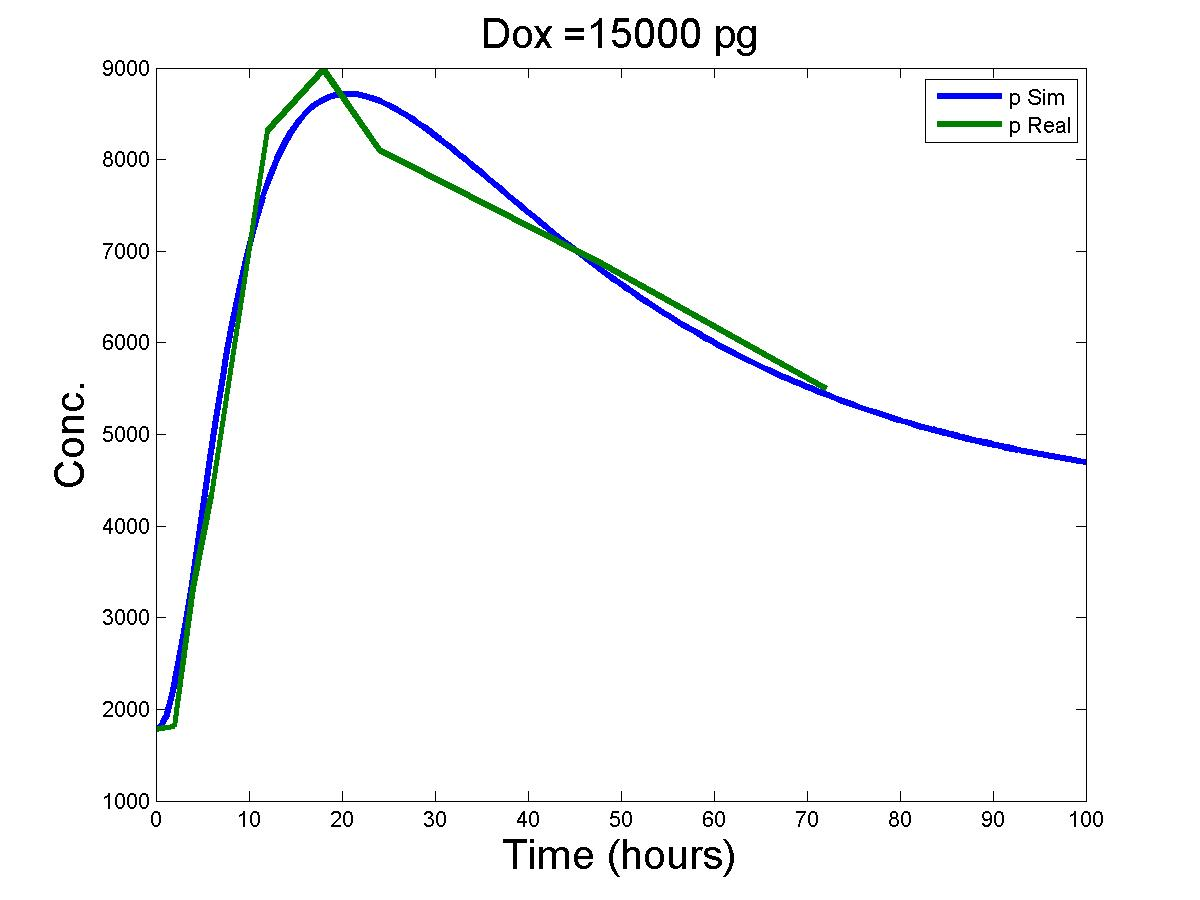
\includegraphics[scale=.1]{MultiDox_pv_mod/Dox15000pCont}}
\subfigure[]{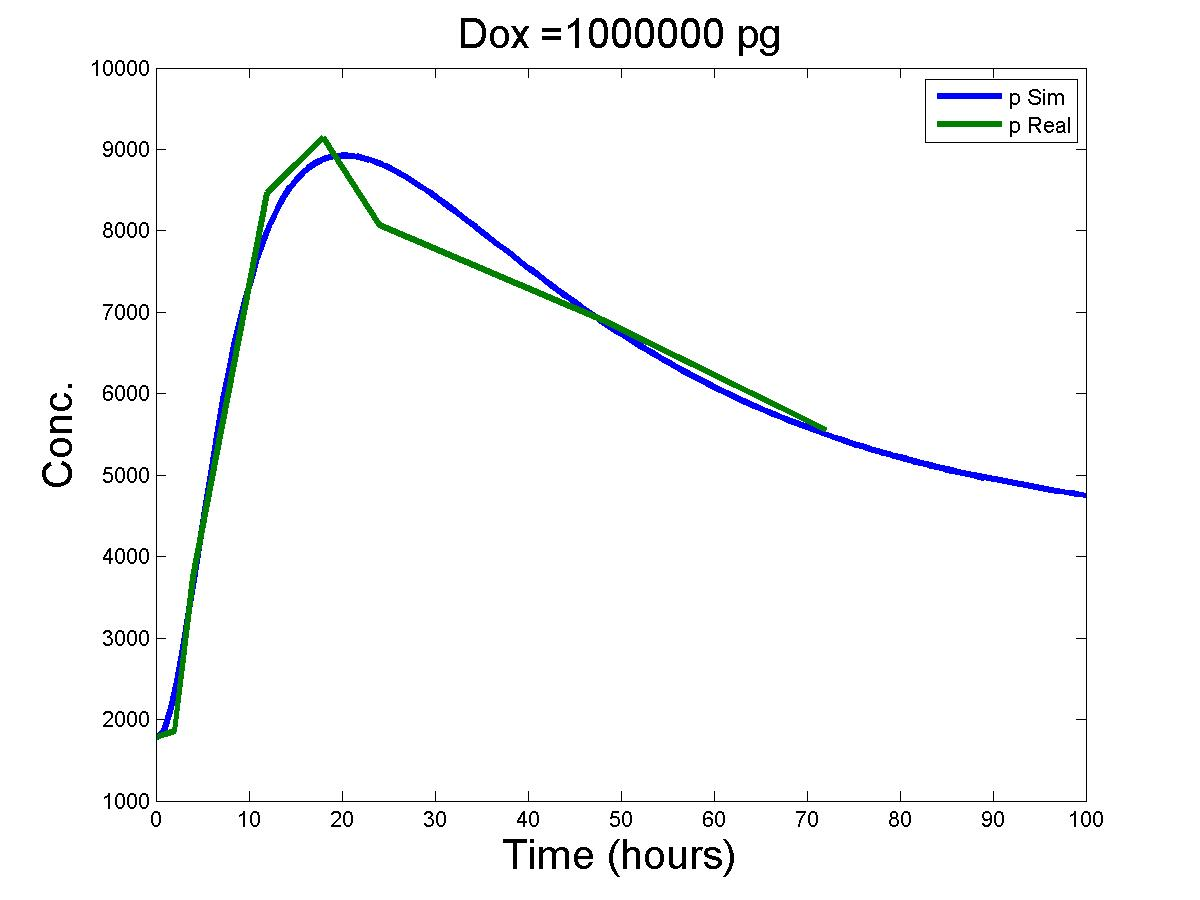
\includegraphics[scale=.1]{MultiDox_pv_mod/Dox1000000pCont}}
\caption{Protein conc. fits at different Dox induction level a)800 ng b)1$\mu g$ c)1.5$\mu g$ d)2$\mu g$ e) 2.5$\mu g$ f)5$\mu g$ g)15$\mu g$ h)1$mg$}
\label{MultiDoxFits}
\end{figure}
\pagebreak

\begin{figure}[h!]
\centering
\subfigure[]{\includegraphics[scale=.15]{MultiDox_pv_mod/multidoxplotmrna}}
\subfigure[]{\includegraphics[scale=.15]{MultiDox_pv_mod/multidoxplot}}
\subfigure[]{\includegraphics[scale=.15]{MultiDox_pv_mod/multidoxplotActualIncl}}
\caption{Predicted plots at different Dox induction levels for a) mRNA b) Protein c) Protein with observed data}
\label{MultiDoxpredict}
\end{figure}

The same is performed for the open loop data. The plots for the
protein fits is seen in Figure~\ref{MultiDoxFitsOpen} for the control cell line. The predicted plot for fluorescence and mRNA levels at different Dox induction levels is shown in the Figure~\ref{MultiDoxpredictOpen}.
\pagebreak

\begin{figure}[h!]
\centering
\subfigure[]{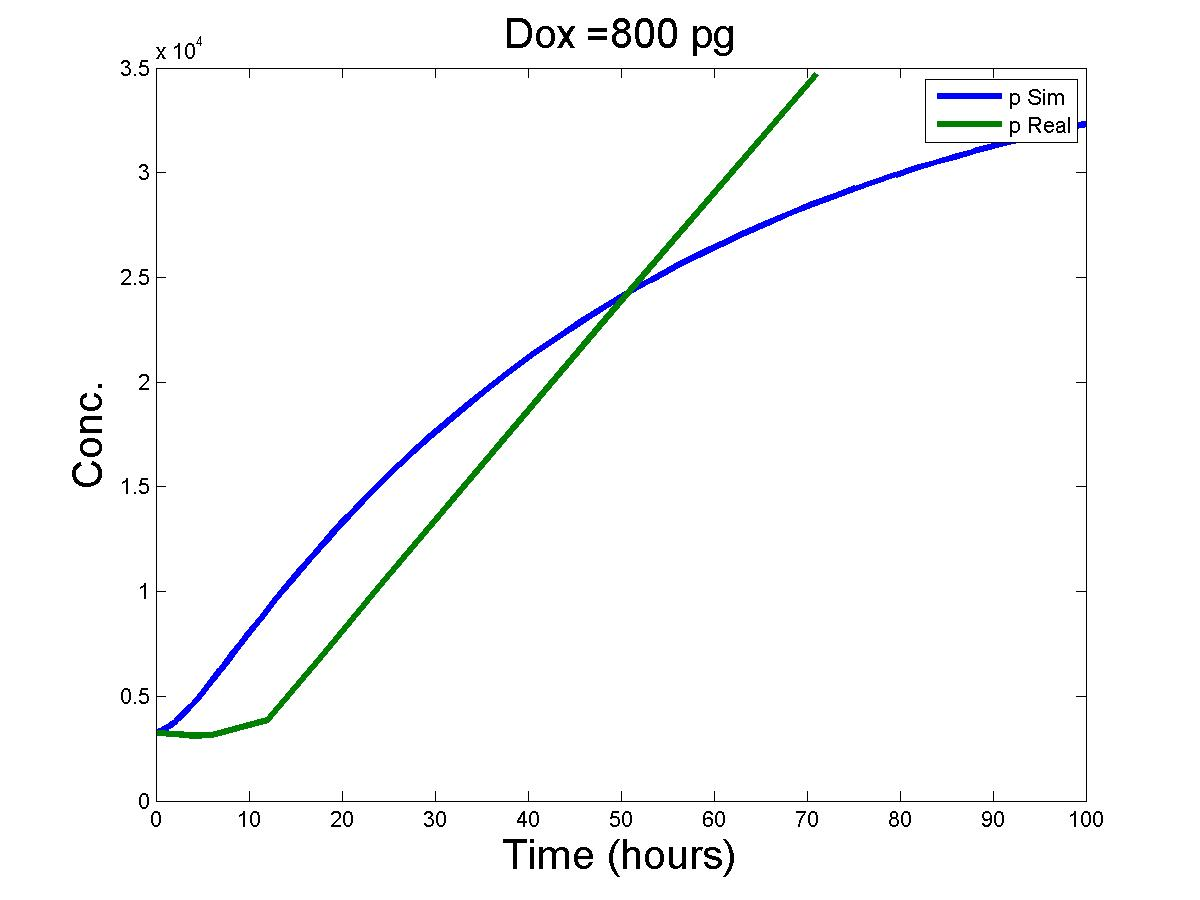
\includegraphics[scale=.1]{MultiDox_p/Dox800pCont}}
\subfigure[]{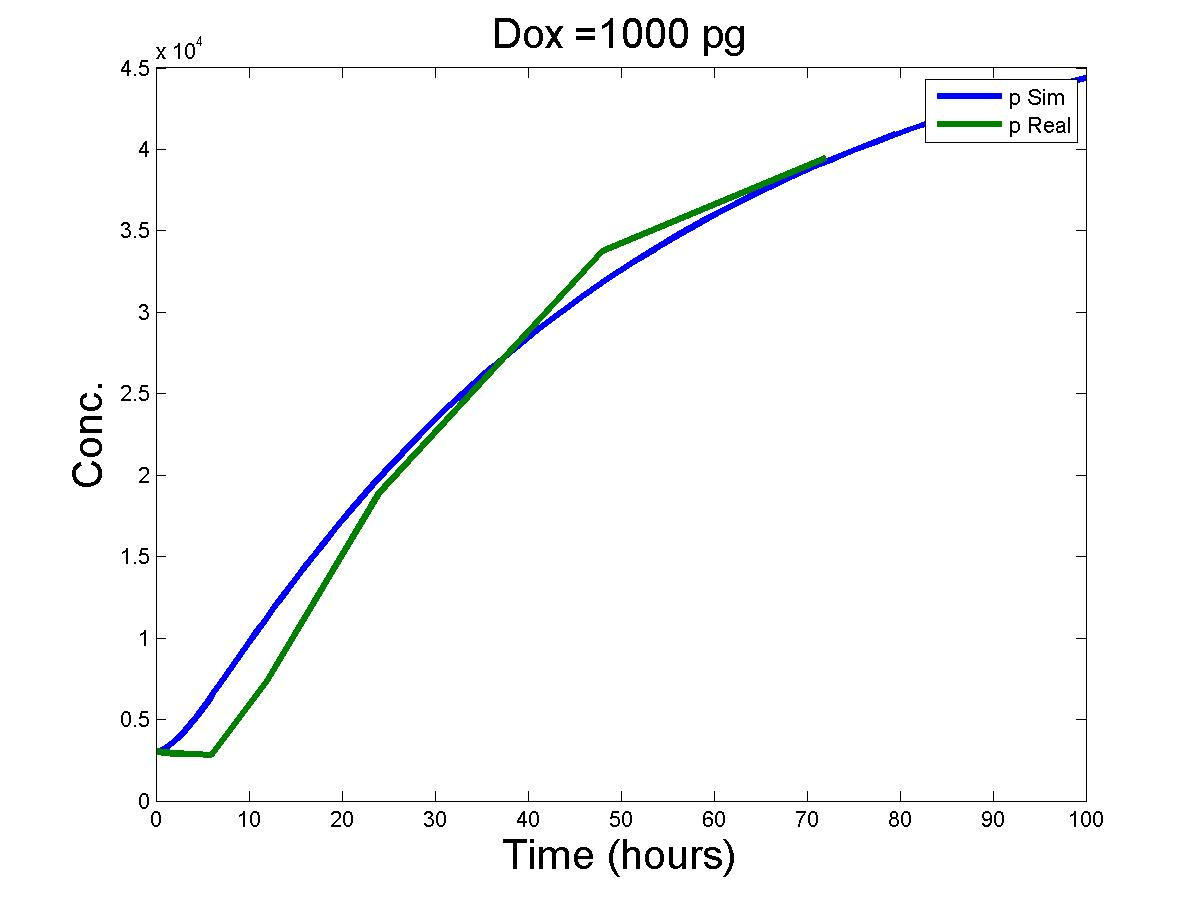
\includegraphics[scale=.1]{MultiDox_p/Dox1000pCont}}
\subfigure[]{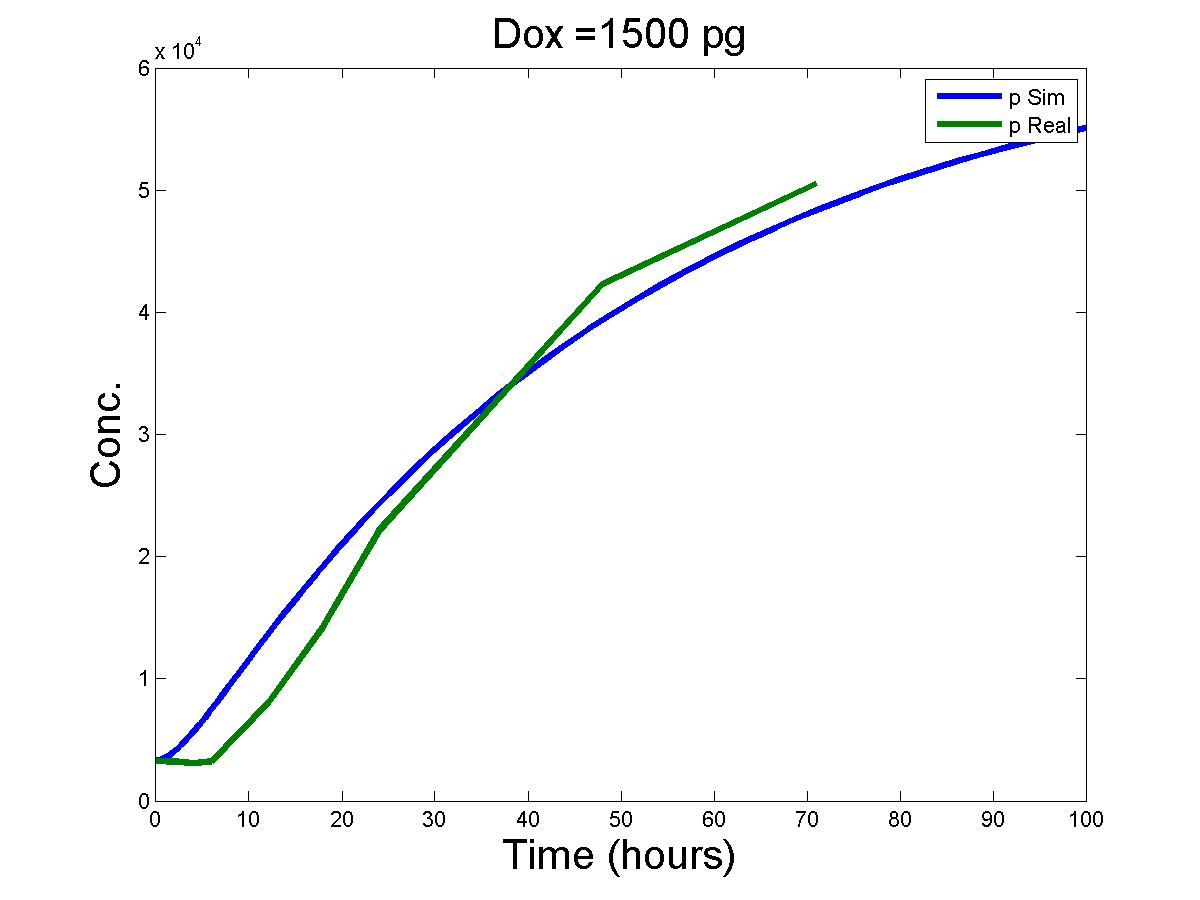
\includegraphics[scale=.1]{MultiDox_p/Dox1500pCont}}
\subfigure[]{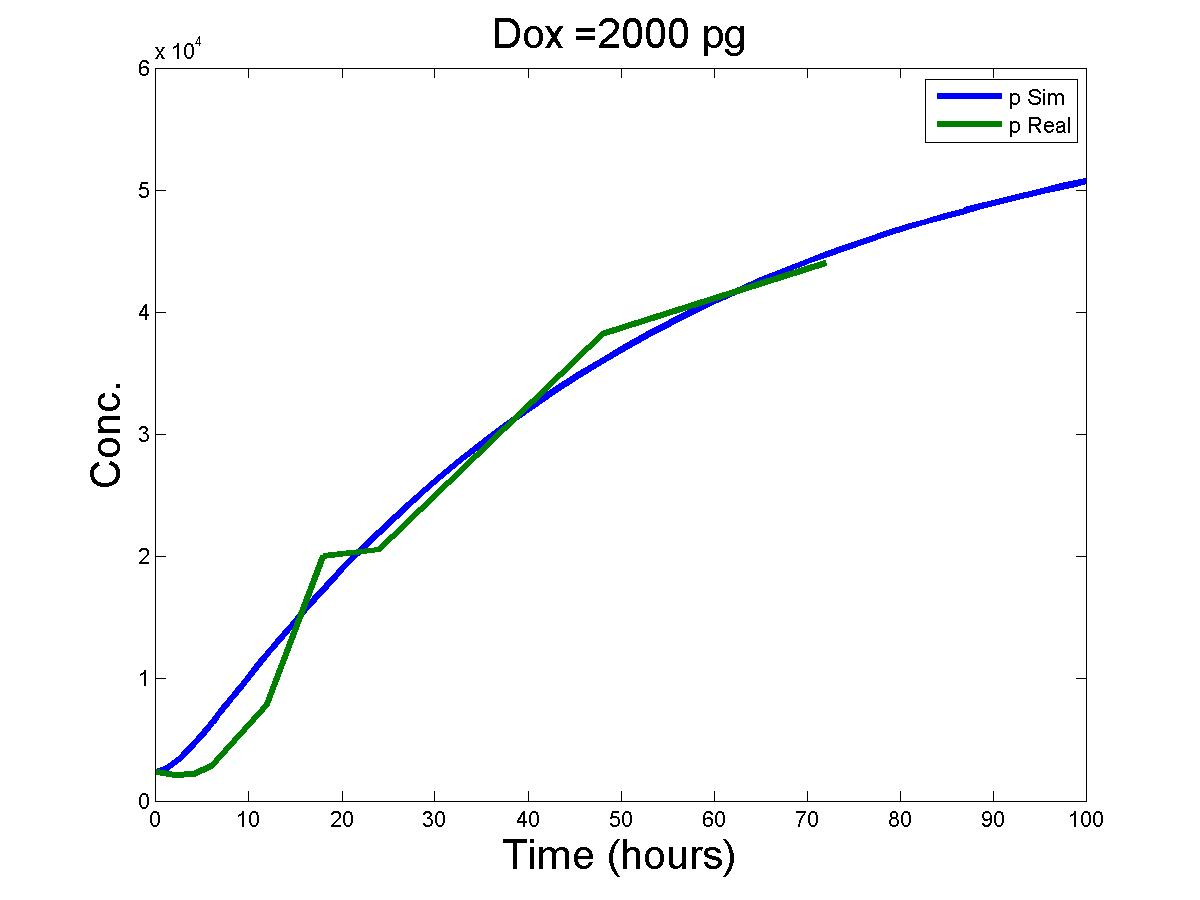
\includegraphics[scale=.1]{MultiDox_p/Dox2000pCont}}
\subfigure[]{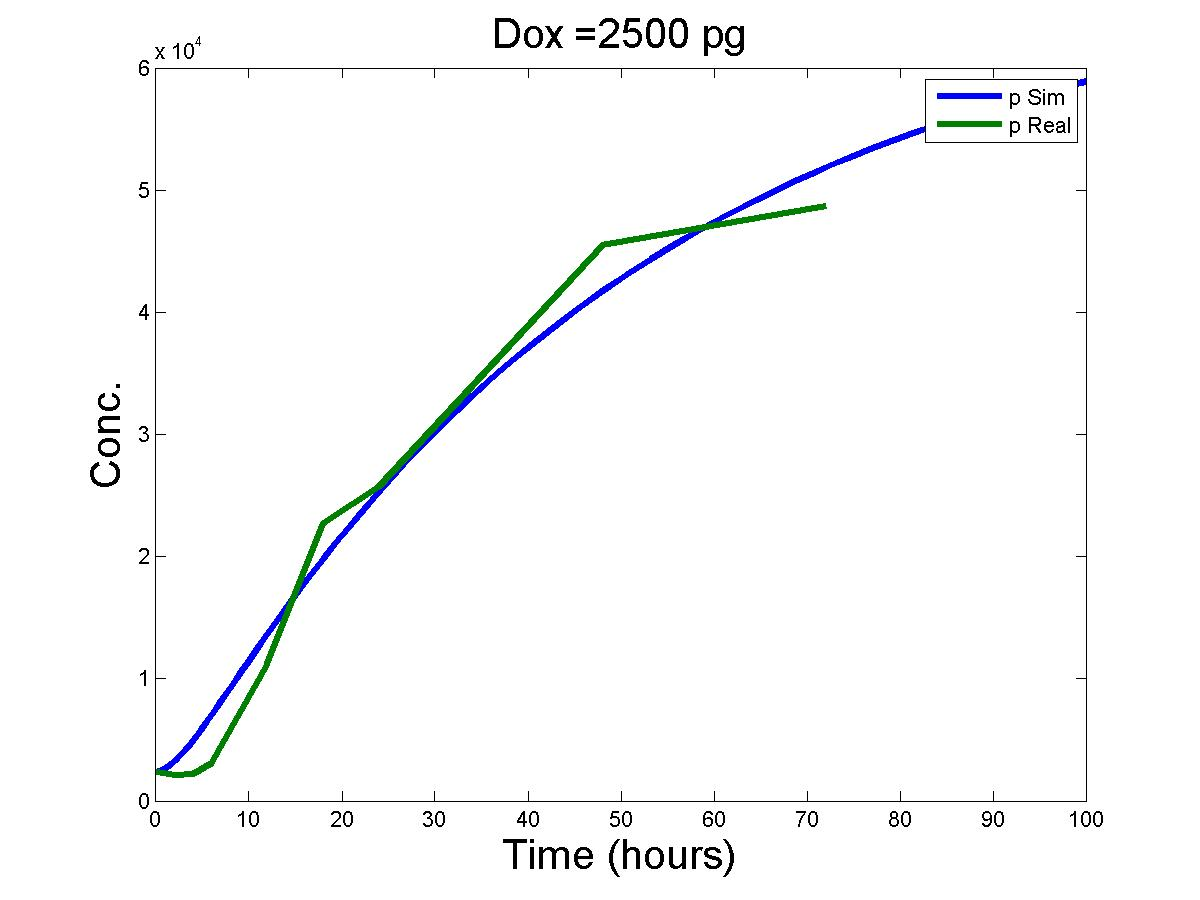
\includegraphics[scale=.1]{MultiDox_p/Dox2500pCont}}
\subfigure[]{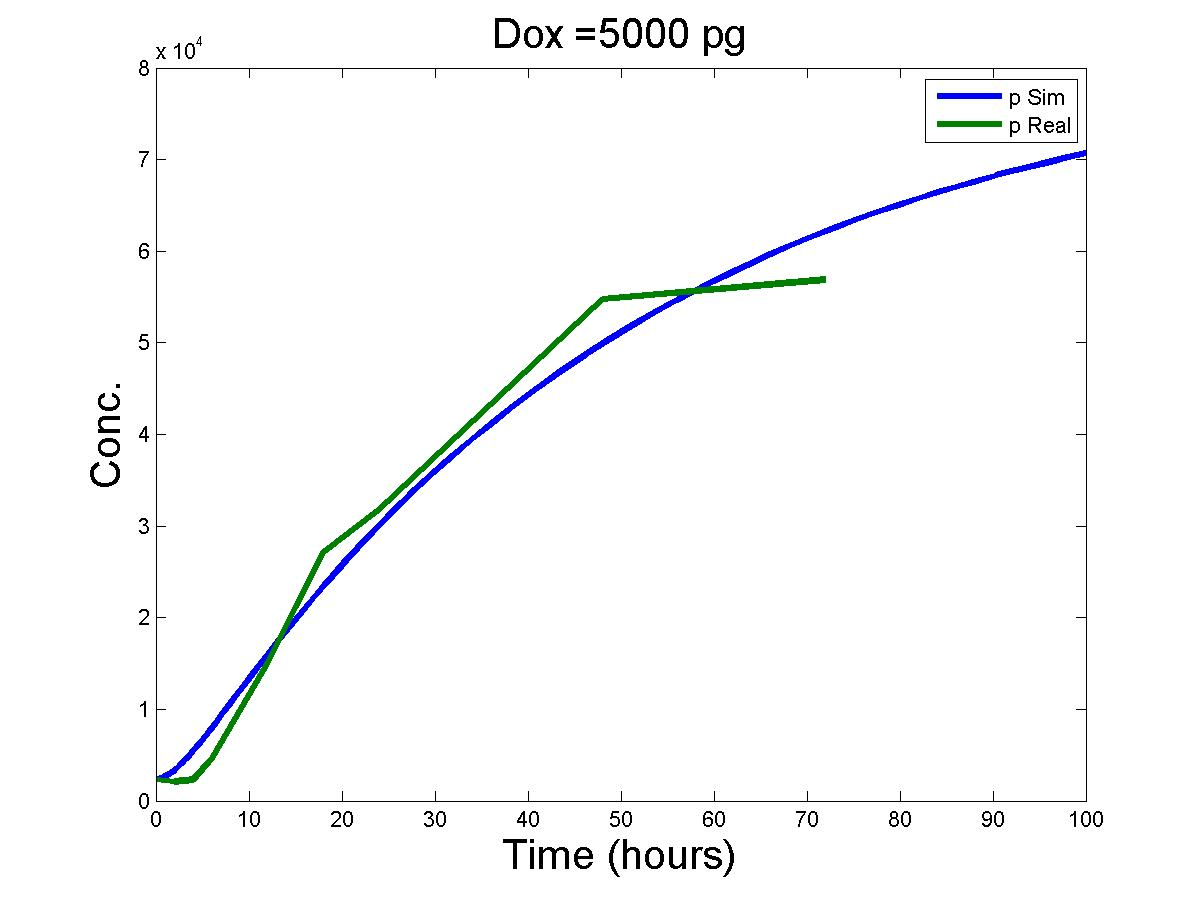
\includegraphics[scale=.1]{MultiDox_p/Dox5000pCont}}
\subfigure[]{\includegraphics[scale=.1]{MultiDox_p/Dox15000pCont}}
\subfigure[]{\includegraphics[scale=.1]{MultiDox_p/Dox1000000pCont}}
\caption{Protein conc. fits at different Dox induction level a)800 ng b)1$\mu g$ c)1.5$\mu g$ d)2$\mu g$ e) 2.5$\mu g$ f)5$\mu g$ g)15$\mu g$ h)1$mg$}
\label{MultiDoxFitsOpen}
\end{figure}
\pagebreak

\begin{figure}[h!]
\centering
\subfigure[]{\includegraphics[scale=.15]{MultiDox_p/multidoxplotmrna}}
\subfigure[]{\includegraphics[scale=.15]{MultiDox_p/multidoxplot}}
\subfigure[]{\includegraphics[scale=.15]{MultiDox_p/multidoxplotActualIncl}}
\caption{Predicted plots at different Dox induction levels for a) mRNA b) Protein c) Protein with observed data}
\label{MultiDoxpredictOpen}
\end{figure}
\pagebreak

The same analysis is now performed on two other cell lines (d3 and d23) and can fe seen in Figures~\ref{MultiDoxFitsd3},~\ref{MultiDoxpredictd3},~\ref{MultiDoxFitsd23},~\ref{MultiDoxpredictd23}.
\begin{figure}[h!]
\centering
\subfigure[]{\includegraphics[scale=.1]{MultiDox_d3/Dox800pCont}}
\subfigure[]{\includegraphics[scale=.1]{MultiDox_d3/Dox1000pCont}}
\subfigure[]{\includegraphics[scale=.1]{MultiDox_d3/Dox1500pCont}}
\subfigure[]{\includegraphics[scale=.1]{MultiDox_d3/Dox2000pCont}}
\subfigure[]{\includegraphics[scale=.1]{MultiDox_d3/Dox2500pCont}}
\subfigure[]{\includegraphics[scale=.1]{MultiDox_d3/Dox5000pCont}}
\subfigure[]{\includegraphics[scale=.1]{MultiDox_d3/Dox15000pCont}}
\subfigure[]{\includegraphics[scale=.1]{MultiDox_d3/Dox1000000pCont}}
\caption{Protein conc. fits at different Dox induction level a)800 ng b)1$\mu g$ c)1.5$\mu g$ d)2$\mu g$ e) 2.5$\mu g$ f)5$\mu g$ g)15$\mu g$ h)1$mg$}
\label{MultiDoxFitsd3}
\end{figure}
\pagebreak

\begin{figure}[h!]
\centering
\subfigure[]{\includegraphics[scale=.15]{MultiDox_d3/multidoxplotmrna}}
\subfigure[]{\includegraphics[scale=.15]{MultiDox_d3/multidoxplot}}
\subfigure[]{\includegraphics[scale=.15]{MultiDox_d3/multidoxplotActualIncl}}
\caption{Predicted plots at different Dox induction levels for a) mRNA b) Protein c) Protein with observed data}
\label{MultiDoxpredictd3}
\end{figure}
\pagebreak

\begin{figure}[h!]
\centering
\subfigure[]{\includegraphics[scale=.1]{MultiDox_d23/Dox800pCont}}
\subfigure[]{\includegraphics[scale=.1]{MultiDox_d23/Dox1000pCont}}
\subfigure[]{\includegraphics[scale=.1]{MultiDox_d23/Dox1500pCont}}
\subfigure[]{\includegraphics[scale=.1]{MultiDox_d23/Dox2000pCont}}
\subfigure[]{\includegraphics[scale=.1]{MultiDox_d23/Dox2500pCont}}
\subfigure[]{\includegraphics[scale=.1]{MultiDox_d23/Dox5000pCont}}
\subfigure[]{\includegraphics[scale=.1]{MultiDox_d23/Dox15000pCont}}
\subfigure[]{\includegraphics[scale=.1]{MultiDox_d23/Dox1000000pCont}}
\caption{Protein conc. fits at different Dox induction level a)800 ng b)1$\mu g$ c)1.5$\mu g$ d)2$\mu g$ e) 2.5$\mu g$ f)5$\mu g$ g)15$\mu g$ h)1$mg$}
\label{MultiDoxFitsd23}
\end{figure}
\pagebreak

\begin{figure}[h!]
\centering
\subfigure[]{\includegraphics[scale=.15]{MultiDox_d23/multidoxplotmrna}}
\subfigure[]{\includegraphics[scale=.15]{MultiDox_d23/multidoxplot}}
\subfigure[]{\includegraphics[scale=.15]{MultiDox_d23/multidoxplotActualIncl}}
\caption{Predicted plots at different Dox induction levels for a) mRNA b) Protein c) Protein with observed data}
\label{MultiDoxpredictd23}
\end{figure}

The comparison of the the steady state protein level with varying levels of Dox induction for the four different cell lines are shown in Fig~\ref{DoxVsSteadyState} :- 
\pagebreak

\begin{figure}[h!]
\centering
\subfigure[]{\includegraphics[scale=.15]{MultiDox_pv_mod/DoxVsProteinIFFL}}
\subfigure[]{\includegraphics[scale=.15]{MultiDox_p/DoxVsProteinIFFL}}
\subfigure[]{\includegraphics[scale=.15]{MultiDox_d3/DoxVsProteinIFFL}}
\subfigure[]{\includegraphics[scale=.15]{MultiDox_d23/DoxVsProteinIFFL}}
\caption{Dox Vs Steady State protein values for a) PV b) P c)d3 d)d23}
\label{DoxVsSteadyState}
\end{figure}

\subsection{Model for $\alpha_m$ variance with induction}
We then hypothesize that the $\alpha_m$ values will have a similar functional relationship with Dox induction levels. For the purpose of the study we assume two models i) $\alpha_m = \frac{a x}{b x + 1}$, ii) $\alpha_m = \frac{a x^n}{b x^n + 1}$. The matlab function 'fit' was used to fit these models. The plots are seen in Figure~\ref{DoxVsAmPred}.    The fits are seen in Figure~\ref{DoxVsAmPred}. 
\pagebreak

\begin{figure}[h!]
\centering
\subfigure[]{\includegraphics[scale=.15]{MultiDox_pv_mod/AmVsDoxPred}}
\subfigure[]{\includegraphics[scale=.15]{MultiDox_p/AmVsDoxPred}}
\subfigure[]{\includegraphics[scale=.15]{MultiDox_d3/AmVsDoxPred}}
\subfigure[]{\includegraphics[scale=.15]{MultiDox_d23/AmVsDoxPred}}
\caption{Dox Vs $\alpha_m$ for a) PV b) P c)d3 d)d23}
\label{DoxVsAmPred}
\end{figure}

\begin{table}[h!]
\begin{center}
\begin{tabular}{|l|l|l|l|l|l|}
\hline
Cell Line & Model Type & a & b & n & SSE \\\hline
PV & Linear & 0.0812 & 5.82e-4 & 1 & 385.5\\\hline
PV & Nonlinear & 0.0053 & 4.04e-5 & 1.3825 & 186.6\\\hline
P & Linear & 0.0798 & 6.644e-4 & 1 & 471.7\\\hline
P & Nonlinear & 0.0241 & 2.061e-4 & 1.17 & 433.7\\\hline
d3 & Linear & 0.205 & 4.61e-4 & 1 & 9913.7\\\hline
d3 & Nonlinear & 0.0114 & 2.73e-5 & 1.405 & 8044.7\\\hline
d23 & Linear & 0.1362 & 5.89 e-4 & 1 & 1183.6 \\\hline
d23 & Nonlinear &0.0031 & 1.42e-5 & 1.53 & 183.3 \\\hline
\end{tabular}
\end{center}
\caption{Parameter Values for $\alpha_m$ Vs Dox plots}
\label{CFam}
\end{table}

\pagebreak

\section{Incorporating Translation Inhibition into Models}

It has been demonstrated in several papers that miRNA's not only bind to mRNA's causing them to degrade but also play a role in translational inhibition. This is demonstrated in Figure~\ref{miRNAtrans}. 
\begin{figure}[h!]
\centering
\includegraphics[scale=.8]{DocPics/miRNAtrans}
\caption{Modes of translation inhibition in miRNAs}
\label{miRNAtrans}
\end{figure}
\subsection{Modeling}
Based on Figure~\ref{miRNAtrans}, miRNA not only causes enhanced mRNA degradation by binding to it but also competes for cap binding and causes ribosome dropoff once they are attached to a mRNA. Both these effects cause the translation rate to decrease for the fraction of mRNA's that are attached to the miRNA's. 


\section{Future Direction}

\begin{itemize}
\item Identify the exact order and mechanism of miRNA based repression 
\item Come up with a mathematical model to capture the translation inhibition 
\item Demonstrate how this could work out to our benefit in synthetic control circuits
\end{itemize}


\end{document}
